\documentclass[12pt]{article}
\usepackage{amsmath}
\usepackage{graphicx}
\date{}
\begin{document}

\tableofcontents
\pagebreak

\section{Introduction}

The work focuses on the relationships between dependent binomial variables, with the intention of modelling K-stage binomial processes and offering improved decision rules for MAB style problems.

So far we have assumed each 'lever' to be a website. Though models could just as well apply to a particular placement or creative.

We hope that the models can be further expanded to include a more complex hierarchy, for example, campaign-site-placement. Or could dependencies on for example, fixed effect regressors for creative or user category.

We provide:
\begin{itemize}
	\item A set of models for dealing with dependent binomial data, including data generation functions.
	\item A set of diagnostic tests for assessing the validity of each model for a novel dataset.
	\item A framework for assessing the usefulness of each model against relevant loss functions for RTB problems.
	\item Decision rules to optimise the explore-exploit trade off in RTB campaigns.
\end{itemize}


\section{Data}

We have 3 vector valued random variables. The ith index represents the values for site domain i for a particular lineitem. In the context on a MAB problem, each index represents a lever. The variables are defined as:
\begin{itemize}
	\item \textbf{n} - number of impressions served over given time period
	\item \textbf{c} - number of clicks on impressions over same time period 
	\item \textbf{a} - number of acquisitions over same time period
\end{itemize}

TODO - bring in relevant sections of EDA document here.

\section{Models}
We define 7 models to fit the data, ultimately intending to model acquisitions.

We start with simple binomial model (m1), then look to beta binomial (m3) to deal with over-dispersion. We then bring in intermediate clicks, hoping these can offer more information on the likelihood of future acqusitions. We find that clicks provide no information on acquisitions unless there is a dependency between p and q. We consider both a cluster model as well as a correlation model to model dependency between p and q.

\subsection{Model 1 - Single Binomial} 
All levers are assumed to have the same payoff function. A useful baseline model. We assume a uniform Beta prior so that the MAP estimate of r is equivlanet to the MLE and is also an unbiased estimator. We gain as much information about lever 1 by looking at lever 2 as by looking at lever 1.

  \begin{align}
	a_i \sim Bin(r,n_i) \\
	\pi(r) = Beta(1,1)
  \end{align}

\subsection{Model 2 - Independent Binomials} 
We assume that each lever has a completely independent payoff function. There is no information to be gained about lever 1 by looking at lever 2.

  \begin{align}
	a_i \sim Bin(r_i,n_i) \\
	\pi(r_i) = Beta(1,1)
  \end{align}

\subsection{Model 3 - Beta-binomial} 
Useful if data is over dispersed for a binomial model. Here we assume a hierarchical model where the conversion rate for each lever is sampled from a Beta distribution with common $\alpha$, $\beta$ parameters across all levers. In a sense, this model lies somewhere between model 1 and model 2, in that data about lever 1 gives us some information about lever 2 via inference of $\alpha$, $\beta$ parameters. 

  \begin{align}
	a_i \sim Bin(r_i,n_i) \\
	r_i \sim Beta(\alpha,\beta) \\
	\pi(\alpha) = Unif(0,10000) \\
	\pi(\beta) = Unif(0,10000)
  \end{align}

\subsection{Model 4 - Beta-binomial plus clicks} 
Since acquisitions are rare events, we try to gain more information about a lever be modelling the click-through-rate separately from the conversions. Similarly to model 3, CTR and CVR have a hierarchical model.

  \begin{align}
	a_i \sim Bin(q_i,c_i) \\
	c_i \sim Bin(p_i,n_i) \\
	q_i \sim Beta(\alpha_q,\beta_q) \\
	p_i \sim Beta(\alpha_p,\beta_p) \\
	\pi(\alpha_q) = Unif(0,10000) \\
	\pi(\beta_q) = Unif(0,10000) \\
	\pi(\alpha_p) = Unif(0,10000) \\
	\pi(\beta_p) = Unif(0,10000) 
  \end{align}

When p and q are independent of each other, $a_i$ has distribution $Bin(p_iq_i,n)$ and $p_iq_i$ has distribution $Beta(a_i,n_i - a_i)$ (see 'Do Clicks Matter' for proof). This makes it equivalent to model 3 with different priors. The intuition here is that clicks are not informative - as much as they increase our belief in click through rate, they decrease our belief in the acquisition rate.

\subsection{Model 5 - 2 cluster Binomial} 

Useful for comparison against model 6.

\subsection{Model 6 - 2 cluster Beta-binomial }

Model 4 assumed that CTR and CVR are independent. Experience suggests that levers tend to perform well on both CTR and CVR or poorly on both. In other words, there tend to be 'clusters' of good and bad levers. Model 5 attempts to capture this with a beta-binomial mixture model. We use priors to bias one cluster towards being the poor performer, this helps avoid 'index switching' complications with model fitting. 
 
 \begin{align}
	a_i \sim Bin(q_i,c_i) \\
	c_i \sim Bin(p_i,n_i) \\
	k \sim Bern(h) 
\end{align}
	\[ 
	q_i \sim 
  	\begin{cases}
		Beta(\alpha_{q0},\beta_{q0}) & \quad \text{if k is 0}\\
		Beta(\alpha_{q1},\beta_{q1}) & \quad \text{if k is 1}
	\end{cases}
	\]
	\[
	p_i \sim 
  	\begin{cases}
		Beta(\alpha_{p0},\beta_{p0}) & \quad \text{if k is 0}\\
		Beta(\alpha_{p1},\beta_{p1}) & \quad \text{if k is 1}\\
	\end{cases}
	\]

 \begin{align}
	\pi(h) = Unif(0,1) \\
	\pi(\alpha_{q0}) = Gamma(1,2) \\
	\pi(\beta_{q0}) = Gamma(1,2) \\
	\pi(\alpha_{p0}) = Gamma(1,2) \\
	\pi(\beta_{p0}) = Gamma(1,2) \\
	\pi(\alpha_{q1}) = Unif(0,10000) \\
	\pi(\beta_{q1}) = Unif(0,10000) \\
	\pi(\alpha_{p1}) = Unif(0,10000) \\
	\pi(\beta_{p1}) = Unif(0,10000)
\end{align}

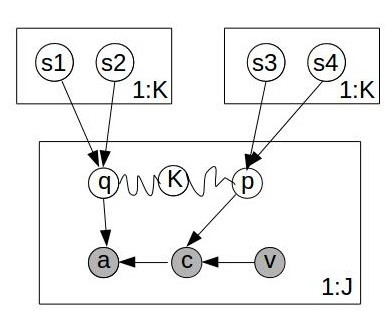
\includegraphics{GraphMod.jpg}

\subsection{Model 7 - Correlated Beta-binomial }

'Bacon With Your Eggs? Applications of a New Bivariate Beta-Binomial Distribution'
'The Use of a Correlated Binomial Model for the Analysis of Certain Toxicological Experiments'
Lee - 'Properties and Applications of the Sarmanov Family of Bivariate Distributions'

As an alternative to model 6, where rate prediction will change abruptly between clusters, we look for a model where q can vary smoothly as a function of p.

We use a relatively unused binomial correlation model, discussed in 'Bacon With Your Eggs? Applications of a New Bivariate Beta-Binomial Distribution'. 

\section{Diagnostic testing}

We take the approach of starting with a simple model and run further tests to decide whether there is evidence to expand the model. 

Where possible we prefer tests with strong theoretical backing, e.g. LR. As model complexity rises it becomes harder to rely on these. We use information criteria and posterior validation.

\subsection{test 1} A frequentist style goodness of fit test designed to assess whether data can be well explained with simple binomial model 1. We use the binomial approximation to the Normal and perform pearson chisq on the residuals. This only holds for large n, so we group the small n values to test whether (together) they share the same mean.

Benefits are that we can have a composite alternative hypothesis, downside is the approximation used. Could be improved by Yates' corerction. TODO - approximation fails for p as rate is very small.

'Goodness-of-Fit Issues in Toxicological Experiments Involving Litters of Varying Size'

\subsection{test 2}

Assuming we reject model 1, we try LR test to see if data is better modelled using beta-binomial. Testing null hypothesis against all others is difficult. LR test has the benefit of being 'most powerful' for comparing 2 point hypotheses, so is a good choice assuming we are happy using ML point hypotheses. If we were willing to specify priors on parameters, we could turn this in to a Bayes factor test.

TODO - compare ratio value to alpha, or do chisq on deviances?

Although this test can show whether Model 3 is better, it can not show whether it is 'good'. This paper has excellent review of goodness-of-fit tests for beta-binomial model:
'Bootstrap goodness-of-fit test for the beta-binomial model'

We use both VGAM and Stan package to get ML estimates for beta-binomial.

\subsection{test 3}

LR test Model 1 vs Model 5 - 1 cluster binomial vs 2 cluster binomial. 

This is a cheap - 'are there clusters between median values' test. 

\subsection{test 4}

Assuming we reject null in test 2, due to some form of over dispersion, we check if can extend this to 2 cluster model with another LR test. Obviously we could keep testing for additional clusters. A more general approach could be to define prior penalizing large number of clusters and use VB or Gibbs to find posterior.

This is a cheap - 'are there clusters between median values' test. 


\subsection{test 5}

Use AIC and BIC for comparison between Model 6 and Model 7. These models aren't nested.

\subsection{Posterior predictive checks}

Similar to the goodness of fit checks, these let us compare our model against observed data. First can use the generating functions to visuallly compare.

\subsubsection{Bayesian p-values}

If we can choose a scalar test statistic, we can produce a p value of realized statistic versus model theoretic probably of the statistic being more extreme than that. Not an obvious candidate.

\subsubsection{Chi-square GoF}

Possibly very useful, need to be careful about the validity of the approximation given some small n.

\section{ Performance testing - static loss functions }

The previous diagnostic tests can help us build a probability model. Ultimately, we are interested in making optimal decisions with a certain loss function. 

We look at the distribution of realized loss functions with k-fold cross validation. And compare the Advance data under each of our proposal models, and benchmark this against the results of the generated data.

We define 4 loss functions:
\begin{enumerate}
	\item Posterior likelihood of realized CVR. 
	\item Difference in conversion rate between estimated top site and true top site.
	\item Volume weighted difference in realized CVR (relates closely to budget wasted). 
	\item Vol weighted MSE.
\end{enumerate}

\section{ Decision rules }

\section{ Performance testing - online }

We now turn this in to the online problem. In contrast to the existing MAB literature, which tends to focus on asymptotic results, we are interested in the performance over finite trials.

We first look at the changes in the realized and expected loss functions, given varying sizes of initial trials. With this, we can estimate the value of exploration. It would be great if we could do this analytically, but I suspect this would be very tricky. 

We will compare this with some theory from Bayesian medical trial design. Given this investigative work, we will provide a framework for generating optimal decisions in the MAB problem. These may be rules specific to the loss function and model, or it may be a framework to generate them computiationally.

We will compare the performance of our decision rules versus common MAB algorithms and online learning algorithms.

\section{Results}

\subsection{Correlation measures}

% latex table generated in R 3.0.2 by xtable 1.7-3 package
% Wed Jul 23 18:50:50 2014
\begin{table}[ht]
\centering
\begin{tabular}{rlrrrrrrrr}
  \hline
 & g & Cor & IWC & logIWCc & RankCor & items & imps & glmcoef & glmsignif \\ 
  \hline
1 & m1 & -0.03 & -0.00 & -0.01 & 0.01 & 1681 & 12946112 & 0.12 & 0.00 \\ 
  2 & m\_1023111 & -0.07 & 0.03 & 0.10 & 0.20 & 191 & 23228621 & -0.03 & 0.19 \\ 
  3 & m3 & -0.07 & -0.02 & -0.13 & -0.09 & 364 & 13079687 & -0.10 & 0.01 \\ 
  4 & m5 & 0.14 & 0.05 & 0.37 & 0.27 & 324 & 12815129 & 0.76 & 0.00 \\ 
  5 & m6 & 0.03 & 0.04 & 0.23 & 0.05 & 319 & 12743695 & 0.22 & 0.00 \\ 
   \hline
\end{tabular}
\end{table}


\subsection{Diagnostic tests}

TODO - cluster test fails to identify model 5.
TODO - vgam library has problems fitting non betabinom cluster data.
% latex table generated in R 3.0.2 by xtable 1.7-3 package
% Wed Jul 23 18:51:42 2014
\begin{table}[ht]
\centering
\begin{tabular}{rlrrrl}
  \hline
 & g & test1\_BinomGoF & test2\_BinomVsBetaBinom & test3\_2ClustBinom & test4\_2ClustBetaBinom \\ 
  \hline
1 & m1 & 1.00 & 1.00 & 1.00 & Error \\ 
  2 & m\_1023111 & 0.00 & 0.00 & 1.00 & Error \\ 
  3 & m3 & 0.00 & 0.00 & 1.00 & Error \\ 
  4 & m5 & 0.00 & 0.00 & 1.00 & Error \\ 
  5 & m6 & 0.00 & 0.00 & 0.00 & 0 \\ 
   \hline
\end{tabular}
\end{table}

\subsection{Performance tests}

\section{Conclusions}

\begin{itemize}
	\item Need to use log values of p.
	\item Clustering based on $a_i$ creates false correlations.
	\item Clustering based on c does not create false correlations.
	\item Using c greater than 0, correlations do not show up. But become stronger for c gt 1, c gt 2. This is because it reduces the noise of all the small-n zero and one values.
	\item Filter based on realized CTR is no use as it does not help with (3). Needs a correlation measure which properly accounts for likelihood weight of response - closest thing is glm.
	\item Binomial GLM does the best job of (4), though does not consider error in dependent variable.
\end{itemize}

\pagebreak

\section{Appendix}

\subsection{Do Clicks Matter}

\subsubsection{Distribution of a conditioned on n}

Firstly note that:

\begin{align}
{w+a \choose w}{n \choose w+a} &= \frac{n!}{(n-w-a)!w!a} \\
	&= \frac{n!(n-a)!}{((n-a)-w)!w!a!(n-a)!} \\
	&=  {n \choose a}{n-a \choose w}
\end{align}

We may construct the probability mass function for a using the conditional distributions:

\begin{align}
p(a|p,q,n) &= \sum_C p(a|q,c)p(c|p,n) \\
 &= \sum_{c=a}^n {c \choose a} p^a(1-p)^{c-a} {n \choose c} q^c (1-q)^{n-c}
\end{align}

Try to pull out a binomial by reparameterizing with $ w = c-a$:

\begin{align}
&= \sum_{w=0}^{n-a} {w+a \choose a} p^a(1-p)^w {n \choose w+a} q^{w+a} (1-q)^{n-w+a} \\
&= {n \choose a} (pq)^a \sum_{c=a}^n {n-a \choose w} ((1-p)q)^w (1-q)^{(n-a)-w} \\
&= {n \choose a} (pq)^a ((1-p)q +  (1-q))^{n-a} \\
&= Binom(a;pq,n)
\end{align}

Ref: http://math.stackexchange.com/questions/626457/conditional-binomials

\subsubsection{Posterior of qp}

We have now established that a is distributed as $Bin(qp,v)$. The question remains whether the uncertainty around the parameterization qp is reduced by modelling q and p separately.

For given a,c,n counts, p and q are independent. We therefore describe their joint density as.

\begin{align}
 f_{P,Q}(p,q) = Beta(p;c,n-c) Beta(q;a,c-a)
\end{align}

Using the same approach as 'Rao, Linear Statistical Inference and its Applications, 3a.3, pg 168' to get the density of pq, apply the following transformation:
\begin{align}
 u(p,q) = qp, \quad v(p,q) = q  \\
 \implies p(u,v) = \frac{u}{v}, \quad q(u,v) = v
\end{align}

\begin{align}
 f_{U,V}(u,v) &= f_{P,Q}(p(u,v),q(u,v)) 
		\frac{\partial p \partial q}{\partial u \partial v} 
		\text{ ,in range }  (u<v<1,0<u<1) \\
 &= Beta(v;c,n-c) Beta(\frac{u}{v};a,c-a) v^{-1} \\
 &= c . v^{c-1} (1-v)^{n-c-1} (\frac{u}{v})^{a-1} (\frac{v - u}{v})^{c-a-1} v^{-1} \\
 &= c . (1-v)^{n-c-1} u^{a-1} (v - u)^{c-a-1}
\end{align}

Now integrate out v. Noting that the integral has the form of a Beta function, we shift and scale the integral with a change of variable.

\begin{align}
\text{Choose }  w &= \frac{v-u}{1-u} \\
f_U(u) &= c.u^{a-1} \int_u^1 (1-v)^{n-c-1} (v - u)^{c-a-1} \mathrm{d}v \\
 &= c.u^{a-1} \int_0^1 ((1-w)(1-u))^{n-c-1} (w(1-u))^{c-a-1} (1-u) \mathrm{d}w \\
 &= c.u^{a-1} (1-u)^{n-a-1} B(n-c,c-a) \\
 &= Beta(u;a,n-a) = Beta(qp;a,n-a) 
\end{align}

\end{document}
